\label{chap3}

This chapter details the parameter identification of the soft robotic system. First, the material properties and dimensions of the soft robotic manipulator are provided. Then, the determination of the soft robots elongation and curvature stiffness is explained by relating pressure to deformation. Consequently, the pressure to force input mapping is detailed. This allows relating deformation to force, which can be used to determine the non-linear stiffnesses. Once these stiffnesses are determined, the experimental determination of the pump dynamics is presented. 


Parameter identification is necessary for model simulation as well as experimental validation. Some parameters such as the soft robot's mass and dimensions were presented in an earlier work \cite{berkers}. Since the soft robotic manipulator is manufactured by an external company, some material properties are classified. To our best knowledge, the Young's Modulus $E$ and Poisson ratio $\gamma$ are those presented in Table (\ref{tab4:parameters}). These properties allow to calculate shear modulus $G$ as $\frac{E}{2(1+\gamma)}$ and bulk modulus $K$ as $\frac{E}{3(1-2\gamma)}$. It is assumed that the robotic manipulator deforms non-linearly following Neo-Hookeon behaviour \cite{Caasenbrood2020StiffnessModel}. For consistency with linear elasticity these moduli are reformulated as $C_{10} = \frac{G}{2}$ and $D_{1} = \frac{2}{K}$ as used for Finite Element Analysis (FEA) \cite{neohookean}. The geometrical properties are presented in Figure \ref{fig3:dim}.


\begin{table}[H]
    \centering
    \caption{Soft robot properties}
    \begin{tabular}{|c|c|c|} \hline
      \textbf{Parameter}   &  \textbf{Value} & \textbf{Unit} \\ \hline
      Mass $m$             &    0.0332       & $[kg]$ \\ 
      Nominal length $L$ &    0.0644       & $[m]$  \\ 
      Width  $w$     &    0.0664    & $[m]$  \\
      Lever length $r$     &    0.01256      & $[m]$  \\ 
      Young's Modulus $E$  &    69           & $[MPa]$\\ 
      Poisson ratio $\gamma$ &    0.45          & $[-]$ \\ \hline
    \end{tabular}
    \label{tab4:parameters}
\end{table}

\begin{figure}[H] 
    \begin{minipage}[b]{0.49\linewidth}
     \centering
    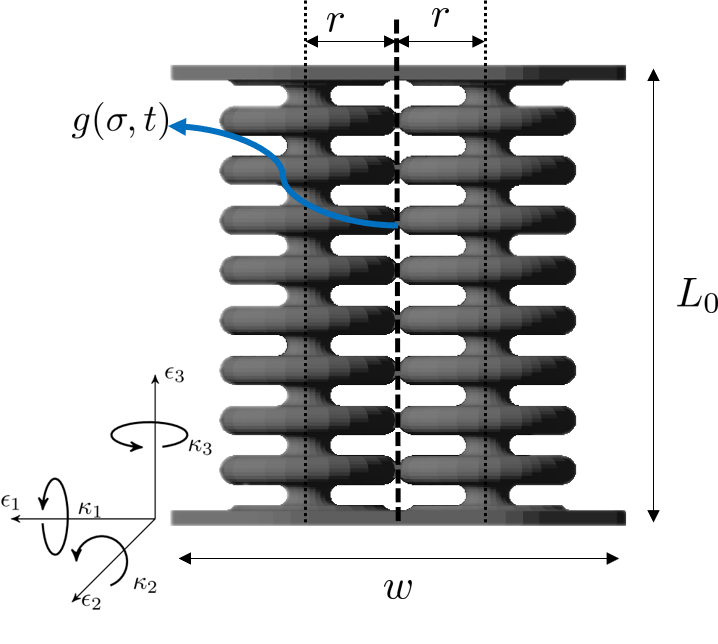
\includegraphics[width=\linewidth]{Figures/Chapter3/dimensions.png} 
    \caption{Schematic overview of the undeformed soft robot with its dimensions.} 
    \label{fig3:dim} 
       \end{minipage} 
    \begin{minipage}[b]{0.49\linewidth}
     \centering
    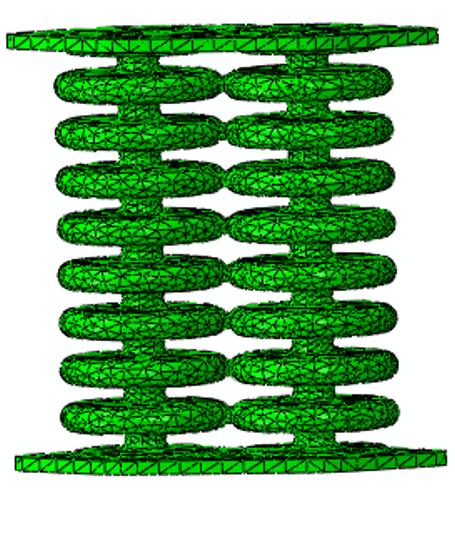
\includegraphics[width=0.7\linewidth]{Figures/Chapter3/undeformed2.png} 
    \caption{Undeformed meshed Finite Element model of the planar robot.} 
    \label{fig3:FemModel} 
    \end{minipage} 
\end{figure}

%%%%%%%%%%%%%%%%%%%%%%%%%%%%%%%%%%%%%%%%%%%%%%%%%%%%%%%%%%%%%%%%%%%%%%%%
%%%%%%%%%%%%%%%%%%%%%%%%%%%%%%%%%%%%%%%%%%%%%%%%%%%%%%%%%%%%%%%%%%%%%%%%
%%%%%%%%%%%%%%%%%%%%%%%%%%%%%%%%%%%%%%%%%%%%%%%%%%%%%%%%%%%%%%%%%%%%%%%%

\section{Finite Element Analysis (FEA)}


In Chapter \ref{chap2} it was derived that two non-linear stiffness's need to be determined. Namely, non-linear curvature stiffness $K_\kappa(\kappa)$ and the elongation stiffness $K_\epsilon(\epsilon)$. To determine these stiffness properties, finite element software \verb+Abaqus/CAE+ is utilized. This software allows studying the deformation of the soft robot under various loads. Stiffness can be approximated by relating applied forces to the magnitude of deformation. To this end, multiple simulations are carried out for a set of bellow pressures. For each of the simulations the modal coordinates $q$ after deformation are obtained. Then, a relation between pressure and force/moment needs to be obtained. This relation is captured by mapping matrix $H$, as was introduced in Chapter \ref{chap2}. The modal coordinates with the mapped pressures can then be used to determine the stiffnesses.

During the analysis we assume no coupling between curvature and elongation, therefore each stiffness can be determined separately. To this end, two different analysis are performed. The first analysis focuses on curvature, while the second analysis targets elongation. Before the outcomes of the analyses are discussed, the FEM model and applied constraints are detailed. Consider Figure \ref{fig3:FemModel} which shows the meshed model used in the finite element software. A mesh refinement analysis is done to determine an accurate mesh size, which is provided in Appendix \ref{app:chap3}. For both analyses, the bottom plate of the actuator is constrained in all directions of motion and rotation. Furthermore, the out-of-plane motion of the actuator is not considered as the body is symmetric and applied loads act perpendicular to this motion. Also, gravitational effects are omitted. First, the curvature analysis and the extraction of the modal coordinates after deformation is considered. Then, the elongation analysis is explained, for which the methodology is analogous. 


\subsection{Curvature analysis}

The curvature analysis allows determining the rotational stiffness of the soft robot. In this analysis, a single bellow is pressurized, whilst the other bellow remains uninflated. The induced pressure causes a moment around the centre of the soft robot. This causes the soft robot to curve and elongate. Figure \ref{fig3:schematiccurvature} shows the deformation the soft robot undergoes during a curvature simulation. The undeformed robot is visualized in blue, the deformed robot is shown in black. In this figure the left bellow is pressurized to 60 kPa.



\begin{figure}[H]
    \centering
\begin{minipage}{0.5\textwidth}
        \centering
        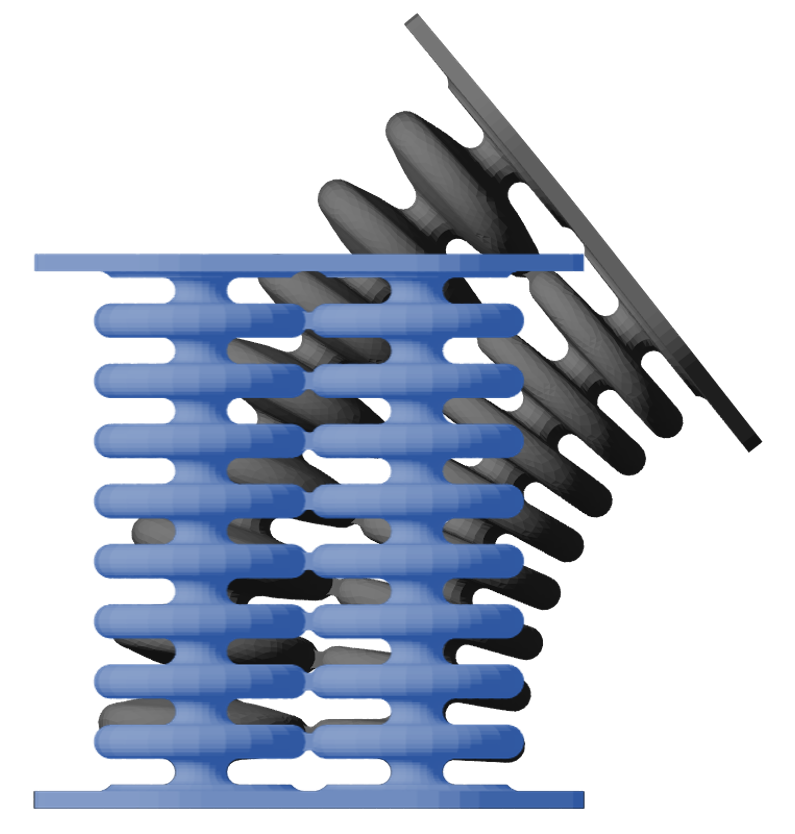
\includegraphics[width=0.695\textwidth]{Figures/Chapter3/curvature.png} 
        \caption{Curvature analysis, undeformed soft robot in blue and deformed robot in black for curvature analysis. }
        \label{fig3:schematiccurvature}
    \end{minipage}\hfill
    \begin{minipage}{0.5\textwidth}
        \centering
        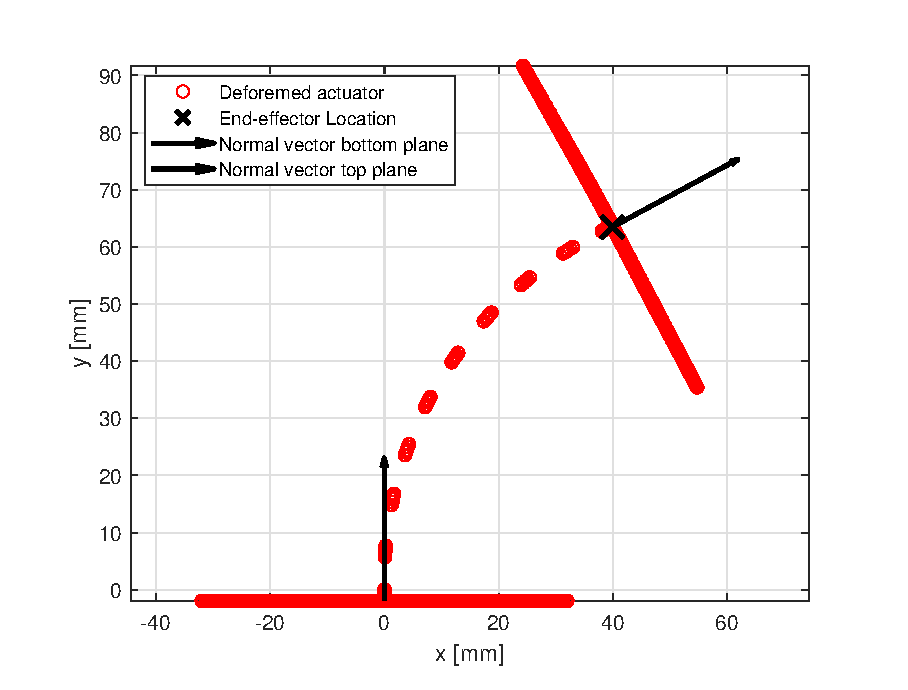
\includegraphics[width=\textwidth]{Figures/Chapter3/rotation60kpa.eps} 
        \caption{Post-processed image of the curvature analysis. The nodes that form the backbone curve clearly isolated.}
        \label{fig3:nodalcurvatrue}
    \end{minipage}
\begin{minipage}{0.5\textwidth}
        \centering
        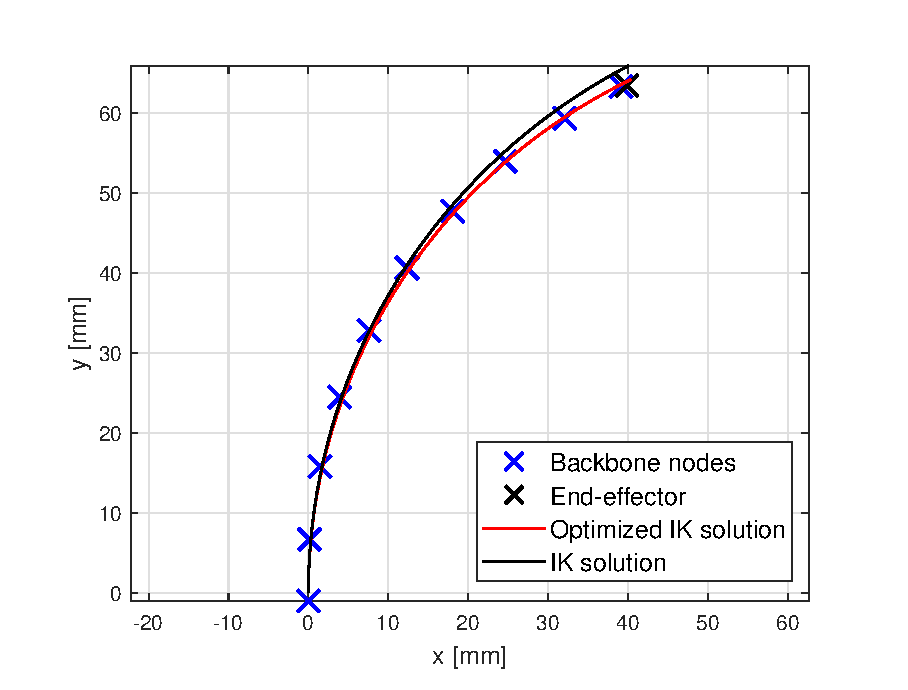
\includegraphics[width=\textwidth]{Figures/Chapter3/rot60kpa.eps}
        \caption{Inverse kinematic fit for an curvature analysis. Left bellow pressurized to 60kPa.}
        \label{fig3:nodalfitcurv}
    \end{minipage}\hfill
    \begin{minipage}{0.5\textwidth}
        \centering
        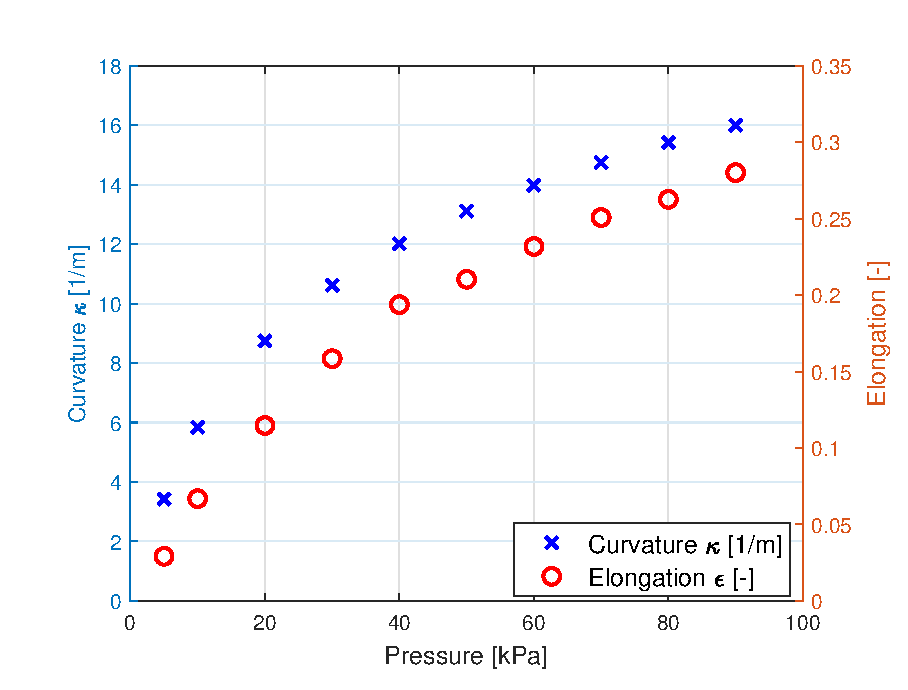
\includegraphics[width=\textwidth]{Figures/Chapter3/curvanalysiscurveps.eps} 
        \caption{Curvature analysis, elongation and curvature as function of pressure.}
        \label{fig3:rotationvspressure}
    \end{minipage}
\end{figure}



After applying loads to the finite element model, nodal displacements can be outputted from $\verb+Abaqus/CAE+$. The acquired data is post-processed in \MATLAB to estimate the elongation and curvature. A post-processed image of the deformation is shown in Figure \ref{fig3:nodalcurvatrue}. This image is created by isolating specific nodes, necessary to reconstruct the backbone curve. In this figure, the top and bottom plate of the robot are visible. Using \MATLAB function \verb+affine_fit.m+ \cite{affinefit} the orientation of both planes with their normal vector can be obtained. Furthermore, this function determines the weighted average of all nodes of the top plate. Which coincides with the end-effector position of the soft robot, $\underbar{r}$. Lastly, the clusters of nodes that are situated at the geometrical mid over the longitudinal axis are isolated. These clusters of nodes are used to reconstruct the backbone curve. 


The post-processed image can be used for kinematic model fitting. This is the last step to obtain modal coordinates $\epsilon$ and $\kappa$ of the deformed soft robot. Figure \ref{fig3:nodalfitcurv} shows this kinematic model fit. Here, the black cross again indicates the end-effector position. Initially, the kinematic fitting is done with the aid of the developed inverse kinematic model as detailed in Appendix \ref{app:chap2}. An inverse kinematic solution can be found based on the end-effector position and rotation. The solution to this kinematic fitting procedure is indicated by the purple curve. This result was deemed insufficiently accurate. Therefore, an optimization method is preferred. This optimization method takes into account the curvature of the entire backbone curve. A total of 10 node clusters are tracked, which can be used to reconstruct the backbone curve. For each cluster of nodes among the backbone the weighted average is calculated, indicated by a blue cross in the figure. The Cartesian position of each of these weighted nodes is given by a vector $s_i \in \mathbb{R}^2$ with $\{i \in \mathbb{N}: i = {1,\dots,10}\}$. Furthermore, the length of the backbone curve is determined by \MATLAB function \verb+arc_length.m+ \cite{arclength}. This functions uses all position vectors $\underbar{$s$}$ to approximate the arc length using splines. This estimated arc length is represented as $\underbar{$l$}_{est} \in \mathbb{R}^+$. The modal coordinates can then be found through optimization with \verb+fmincon.m+. The minimization problem that follows is,


\begin{equation}
\begin{aligned}
\min_{q} \hspace{5pt}  q^\top Q q  + \sum_{i=1}^{10}\Big(\psi_1 ||\text{\underbar{$s$}}_{i} - f(q)_{s,i)})|| \Big) +   \psi_2(\text{\underbar{$r$}}  - f(q)_{r})^2 +  \psi_3(\text{\underbar{$l$}}_{est} - & f(q)_l)^2  \\ 
\text{s.t.} \hspace{5pt} \epsilon - 1 > 0
\end{aligned}
\label{eq3:optim}
\end{equation}


where $f(q)$ is a function describing the forward kinematics based on modal coordinates $q$. Subscripts $s,i$ and $r$ correspond to the position of each node among the backbone curve and end-effector position, respectively. Scalar $f(q)_l \in \mathbb{R}^+$ is the estimated length based on the output of function $f(q)$. Furthermore, $Q$ is $\text{diag}([0.001,0.001])$ is a weighing matrix used to penalize the value of the modal coordinates. Additional weighing factors $\psi = [5e4,5e4,1e4]^\top$ are applied to penalize individual terms. These weighing factors are used to scale individual error terms, and stress relative importance. The only imposed constraint affects the elongation of the soft robot. Physically this constraint implies that the robot can shorten in length, but the length can not become negative. As a note, for a single shape-function approximation, solving the minimization problem only results in slightly better modal coordinate estimates. For studying more complex deformations, that involve estimations with multiple shape functions, this optimization is necessary. An inverse Jacobian search singularly based on end-effector position will not suffice. Some reconstruction of the backbone curve is necessary for such cases. The modal coordinates belonging to the deformation of Figure \ref{fig3:nodalfitcurv} found through optimization are $q = [\kappa,\epsilon]^\top = [-14,0.24]^\top$, which corresponds to an elongation of 24\% and curvature of 14$\frac{1}{m}$ in clockwise direction.


The above-described inverse kinematic optimization is repeated for multiple simulations conducted at different bellow pressures. The results are displayed in Figure \ref{fig3:rotationvspressure}. Here, the obtained curvature and elongation are plotted as a function of bellow pressure. It can be seen that the curvature and elongation rates increase by increments in pressure. Also, the non-linear relation between pressure and deformation is visible..




\subsection{Elongation analysis}
\label{subsecelong}

The elongation analysis aims to measure the elongation of the soft robot. An elongation is induced by pressurizing both bellows equally. This allows determining the elongation stiffness, as the magnitude of rotation of the soft robot is small. Figure \ref{fig3:schematicelong} shows the deformation that the soft robot undergoes during an elongation experiment. Again, the undeformed soft robot is visualized in blue. For the soft robot in black, both bellows are pressurized to 60 kPa. 

Analogous to the curvature analysis, a post-processed image of the deformation is shown in Figure \ref{fig3:nodalelong}. The optimization of (\ref{eq3:optim}) is carried out, to determine modal coordinates. The results of this optimization are shown in Figure \ref{fig3:nodalfitelong}. The modal coordinates belonging to this fit are $q = [\kappa,\epsilon] = [0.06, 0.45]^\top$, showing a negligible curvature and elongation of 45\%. Furthermore, this figure shows that for elongation analysis, the developed inverse kinematic algorithm (Appendix \ref{app:chap2}) already yields decent results.  

Repeating this analysis for a set of 10 different pressures, allows to obtain a relation between elongation and pressure. The results are presented in Figure (\ref{fig3:elongationvspressure}). Additionally, the found curvature is plotted for the pressure range. It is clear that pressurizing the bellows equally results in a near pure elongation. The maximum obtained curvature is equal to 0.07 $\frac{1}{m}$, which is equivalent to a rotation of the upper flange of just 0.32 degrees. This allows determining the elongation stiffness as effects of rotation are deemed negligible. The elongation rate decreases as pressure increases, as a result of the non-linear material parameters. Furthermore, the decoupling between curvature and elongation can be seen. Pressurizing both bellows to 90 kPa results in an elongation of $0.55 [-]$. The curvature analysis showed an elongation of $0.27 [-]$, where only single bellow was inflated. As expected these obtained values differ about a factor 2. 



\begin{figure}[H]
    \centering
\begin{minipage}{0.5\textwidth}
        \centering
        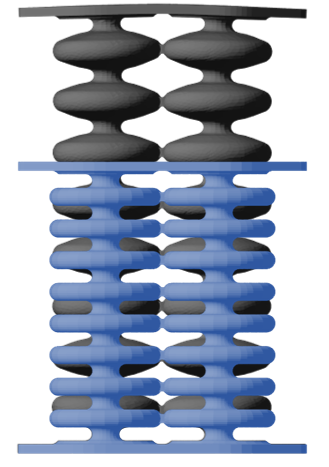
\includegraphics[width=0.53\textwidth]{Figures/Chapter3/elongation.png} 
        \caption{Elongation analysis, undeformed soft robot in blue and deformed robot in black. }
        \label{fig3:schematicelong}
    \end{minipage}\hfill
    \begin{minipage}{0.5\textwidth}
        \centering
        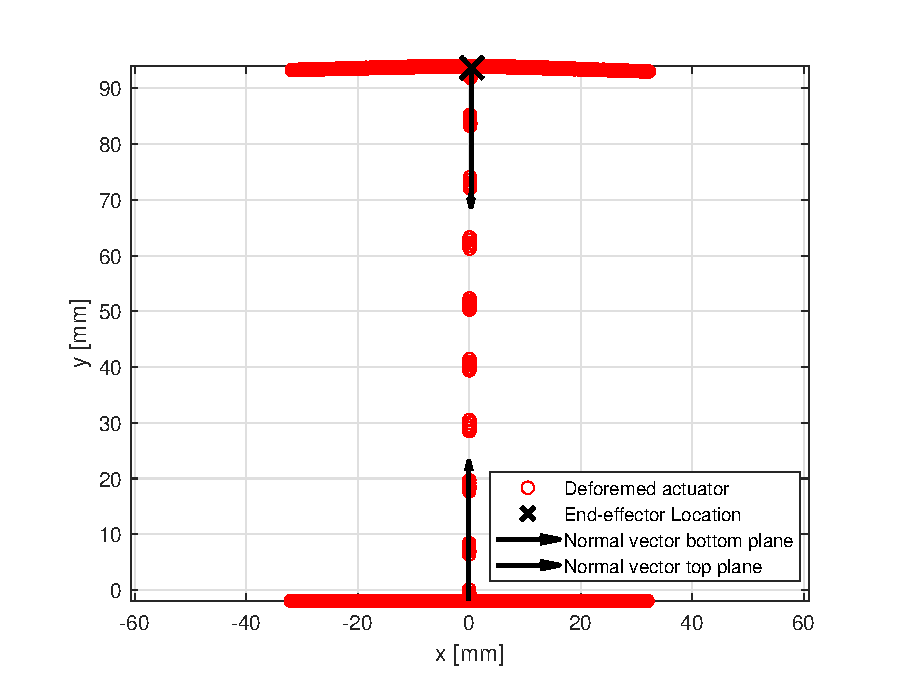
\includegraphics[width=\textwidth]{Figures/Chapter3/elongation60good.eps} 
        \caption{Post-processed image of an elongation analysis. The nodes that form the backbone curve clearly isolated.}
        \label{fig3:nodalelong}
    \end{minipage}
\begin{minipage}{0.5\textwidth}
        \centering
        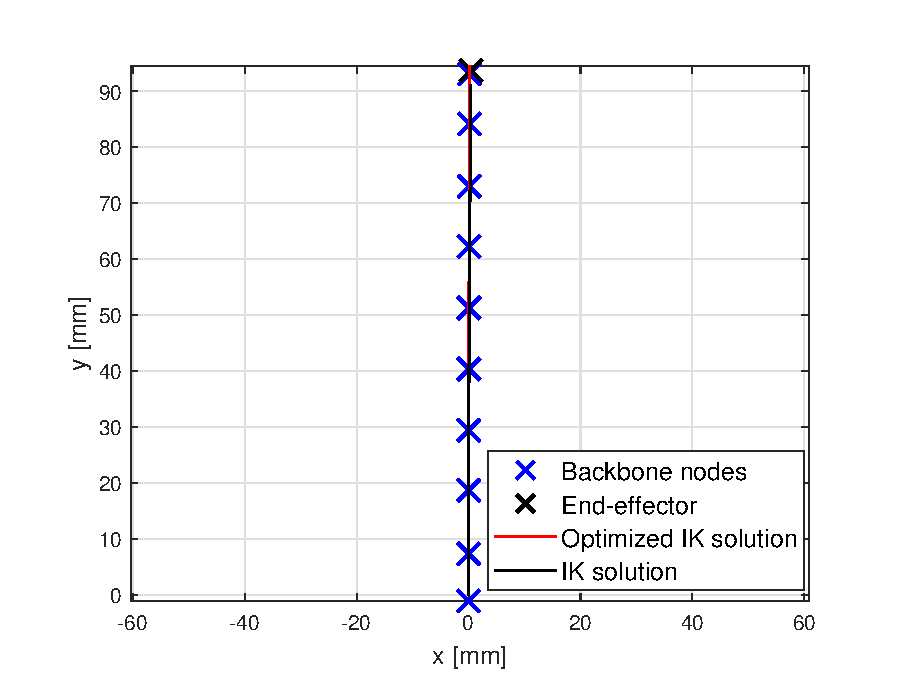
\includegraphics[width=\textwidth]{Figures/Chapter3/elong60kpa.eps}
        \caption{Inverse kinematic fit for an elongation analysis. Both bellows pressurized to 60kPa.}
        \label{fig3:nodalfitelong}
    \end{minipage}\hfill
    \begin{minipage}{0.5\textwidth}
        \centering
        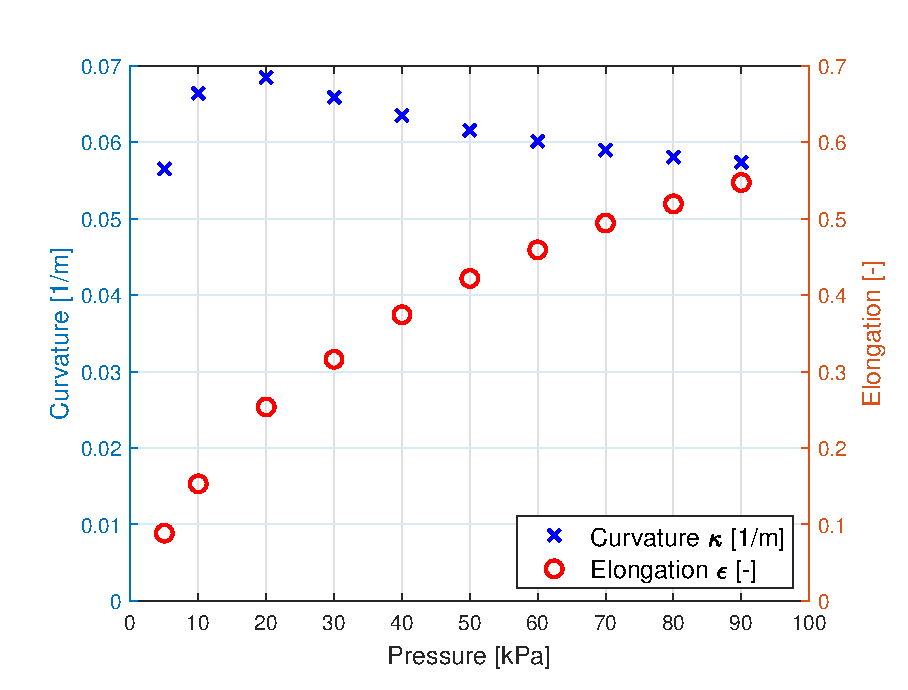
\includegraphics[width=\textwidth]{Figures/Chapter3/elonganalysiscurveps.eps} 
        \caption{Elongation analysis, elongation and curvature as function of pressure. As can be seen curvature is negligibly small.}
        \label{fig3:elongationvspressure}
    \end{minipage}
\end{figure}


At this point, the modal coordinates as a function pressure are derived. However, to determine the stiffness this pressure needs to be mapped to a force and moment. This is discussed in Section \ref{sec3:InputMapping}.



%%%%%%%%%%%%%%%%%%%%%%%%%%%%%%%%%%%%%%%%%%%%%%%%%%%%%%%%%%%%%%%%%%%%%%%%
%%%%%%%%%%%%%%%%%%%%%%%%%%%%%%%%%%%%%%%%%%%%%%%%%%%%%%%%%%%%%%%%%%%%%%%%
%%%%%%%%%%%%%%%%%%%%%%%%%%%%%%%%%%%%%%%%%%%%%%%%%%%%%%%%%%%%%%%%%%%%%%%%



\section{Input Mapping}
\label{sec3:InputMapping}

Stiffness is the ratio between applied force and elongation. To determine stiffness for elongation and curvature, applied forces and direction of deformation is necessary. For the physical system, the individual bellow pressure can be regulated. Therefore force input vector $\nu(p)$ is mapped to pressure by some mapping matrix $H \in \mathbb{R}^{2 \times 2}$, as discussed in Chapter \ref{chap2}. The relation between force input and pressure is given as, 

\begin{equation}
   \nu(p) =   \begin{bmatrix} M \\ F \end{bmatrix}     = \underbrace{\begin{bmatrix}  H_{1,1} & H_{1,2} \\ H_{2,1} & H_{2,2} \end{bmatrix}}_{H}         \begin{bmatrix}  p_1 \\ p_2 \end{bmatrix}, \label{eq3:H}
\end{equation}

where the entries of $H$ are to be determined. The intention is to decouple rotation and elongation. Therefore, it is important to understand that $M$ acts as a moment causing the soft robot to curve. Whereas, $F$ is a force resulting in elongation. This implies that the entries of $H_{1,1}$ and $H_{1,2}$ represent an effective surface area multiplied by the lever on which the force acts. Entries $H_{2,1}$ and $H_{2,2}$ represent an effective surface area. Due to symmetry properties it must hold that $H_{2,1} = H_{2,2}$ and $H_{1,1} = -H_{1,2}$.

First, the relation between pressure and force tried to be obtained. This will be done by using the finite element software again. The idea is to map pressure to force using elongation. Pressurizing both bellows equally, resulted in almost ``pure" elongation. Effectively, the same deformation can be achieved by applying an equally distributed force on the top plate of the actuator. To this end, simulations for a set of forces applied to the upper flange of the soft robot are simulated. This FEA follows the same procedure as for the elongation analysis as discussed in Section \ref{subsecelong}. The results for this simulation are presented in Figure (\ref{fig3:forcemap}). The horizontal axis shows the modal coordinates, determined using the inverse kinematic optimization as discussed previously. The markers in blue correspond to the modal coordinates found for the elongation analysis. The red markers indicate modal coordinates as found by the force analysis. It is clear that pressurizing both bellows or a distributed force on the upper flange result in a comparable deformation. The scaling of the vertical axis already reveals that a linear relation can be found.


\begin{figure}[H]
    \centering
\begin{minipage}{0.5\textwidth}
        \centering
        \includegraphics[width=\textwidth]{Figures/Chapter3/forcepressuremodal.eps}
        \caption{Modal coordinates $\kappa$ and $\epsilon$ for elongation analysis and force analysis.}
        \label{fig3:forcemap}
    \end{minipage}\hfill
    \begin{minipage}{0.5\textwidth}
        \centering
        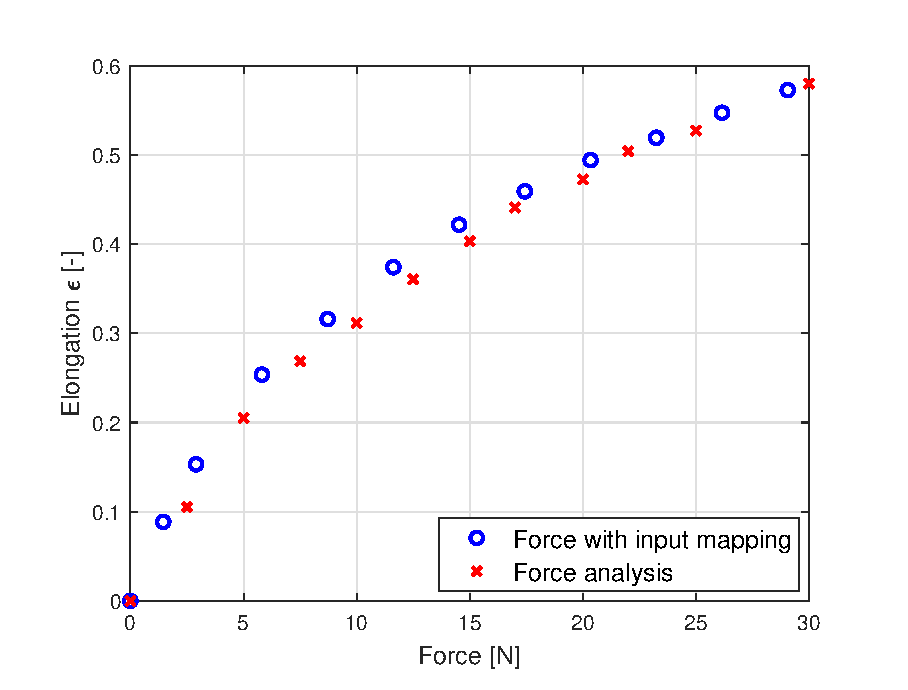
\includegraphics[width=\textwidth]{Figures/Chapter3/pressureforceelongation.eps} 
        \caption{Elongation expressed for force analysis and force with input mapping.}
        \label{fig3:forcetopressure}
    \end{minipage}
\end{figure}
\newpage

The linear mapping coefficient, which maps the pressure to a force, can be found by solving a least squares problem as,

\begin{equation}
\min_{H_{2,2}} \sum_{i=1}^{12} (F_i - 2 H_{2,2} p_i)^2
\label{eq3:forcefitting}
\end{equation}

where $i$ indicates each sample point of the total 12 sample points. The effective pressure area is found to be equal to 0.1462 $m^2$. Since $H_{2,1} = H_{2,2}$ the mapping of pressure in kPa to force in Newton is obtained. Figure (\ref{fig3:forcetopressure}) shows the results of the input mapping for the elongation. It can be seen that the pressure maps fairly accurate to the force.

Now the effective pressure area has been determined, the mapping to the moment can be calculated. It is assumed that the force acts on the top plate at a given radius from the backbone curve. The lever on which the force acts is equal to 12.56 $mm$, as can be seen in Figure \ref{fig3:dim}. This allows to calculate $H_{1,1}$ and $H_{2,1}$ by multiplying $H_{2,1}$ with the radius $r$. The mapping matrix $H$ that follows is given as,

\begin{equation}
    H =  \begin{bmatrix} 1.8245e-3 & -1.8245e-3 \\
    0.14526 & 0.14526\end{bmatrix}.  
\end{equation}

At this point, the modal coordinates for the deformed soft robot for curvature and elongation analysis have been determined. Furthermore, the mapping from pressure to force and moment is derived. Combining the analysis results with this mapping, allows deriving the curvature and elongation stiffness of the soft robot. 

%%%%%%%%%%%%%%%%%%%%%%%%%%%%%%%%%%%%%%%%%%%%%%%%%%%%%%%%%%%%%%%%%%%%%%%%
%%%%%%%%%%%%%%%%%%%%%%%%%%%%%%%%%%%%%%%%%%%%%%%%%%%%%%%%%%%%%%%%%%%%%%%%
%%%%%%%%%%%%%%%%%%%%%%%%%%%%%%%%%%%%%%%%%%%%%%%%%%%%%%%%%%%%%%%%%%%%%%%%



\section{Stiffness properties}

The force mapping and the modal coordinates obtained through inverse kinematic optimization can be utilized to determine elongation and curvature stiffness. A non-linear trend in elongation and curvature as a function of pressure was already observed. Therefore, it is assumed that the stiffness can be captured by the hyper-elastic stiffness model as formulated in \cite{Caasenbrood2020StiffnessModel}. This non-linear stiffness model poses that stiffness $K(q_i) \in \mathbb{R}^{\geq 0}$ and meets condition $K_{min} < K(q_i) < K_{max}$. This means that the actuator stiffness is asymptotic to $K_{max}$ and $K_{min}$.  The elongation stiffness is given by,

\begin{equation}
    K_\epsilon(\alpha,\epsilon) =  \alpha_1 + \alpha_2 [\tanh({\alpha_3 \epsilon})^2 -1],
\end{equation}


where $\alpha \in \mathbb{R}^3$ are positive stiffness parameters to be found. It is assumed that negative pressures, e.g. creating a vacuum, result in equal elongation yet in opposite direction. Hence, the amount of sample points is doubled. The stiffness parameters can be found by solving the non-linear constraint optimisation described by,


\begin{equation}
\begin{aligned}
\min_{\alpha_1,\alpha_2,\alpha_3} \hspace{5pt} \sum_{i=1}^{23}\Big(F_i -  (\alpha_1 + \alpha_2 [\tanh({\alpha_3 \epsilon_i})^2 -1])\epsilon_i\Big)^2    \\ 
\text{s.t.} \hspace{5pt} \alpha_1 > \alpha_2 > 0 \\
\alpha_3 > 0 \\ ,
\label{eq3:Keopt}
\end{aligned}
\end{equation}

which objective is to minimize the sum of the errors between the mapped force, and force resulting from the stiffness model based on the elongation. The results of this optimization are shown in Table \ref{tab3:stiffnessparameters}.

In determining the curvature stiffness the procedure is repeated. Consider the curvature stiffness given by,

\begin{equation}
    K_\kappa(\beta,\kappa) =  \beta_1 + \beta_2 [\tanh({\beta_3 \kappa})^2 -1],
\end{equation}

where $\beta \in \mathbb{R}^3$ contains positive stiffness parameters. Likewise, these parameters can be found by solving,

\begin{equation}
\begin{aligned}
\min_{\beta_1,\beta_2,\beta_3} \hspace{5pt} \sum_{i=1}^{23}\big(M_i -  (\beta_1 + \beta_2 [\tanh({\beta_3 {\kappa_i}})^2 -1]){\kappa_i}\Big)^2    \\ 
\text{s.t.} \hspace{5pt} \beta_1 > \beta_2 > 0 \\
\beta_3 > 0 \\ 
\label{eq3:Kkopt}
\end{aligned}
\end{equation}

where the objective is to minimize the sum of errors between the mapped moment and the curvature stiffness as given by the model. The resulting stiffness of this optimization is also shown in Table (\ref{tab3:stiffnessparameters}). 

\begin{table}[H]
    \centering
        \caption{Parameters for hyper-stiffness model.}
\begin{tabular}{|c|c|c|c|} \hline
            &  $i = $ 1      &    $i = $    2   &  $i = $ 3  \\ \hline
   $\alpha_i \hspace{2pt}[N]$    &    1.3936e+3    & 1.3776e+3    & 2.7865e-1 \\ \hline
   $\beta_i \hspace{2pt}  [Nm^2] $     &  3.0322 & 3.0309    &  3.3755e-3\\ \hline
\end{tabular}
    \label{tab3:stiffnessparameters}
\end{table}

The stiffness model can be plotted as a function of applied force and moment. These results are shown in Figure \ref{fig3:elongvsforce} and \ref{fig3:curvsmoment} for force and moment, respectively. The model shows that force and moment applied for the FEA analysis well correspond to the obtained stiffness function. 


\begin{figure}[H]
    \centering
\begin{minipage}{0.5\textwidth}
        \centering
        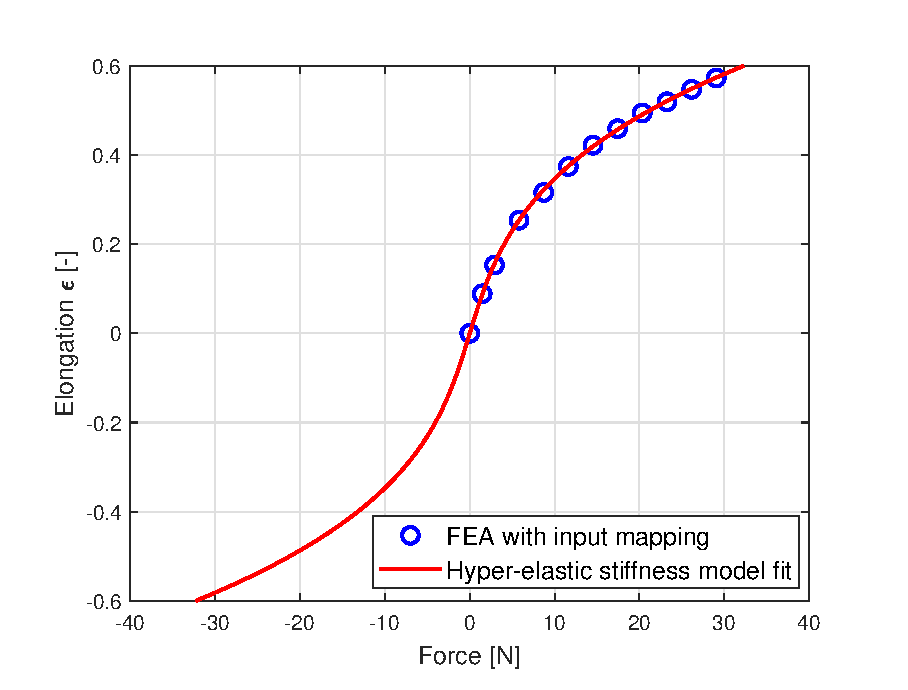
\includegraphics[width=\textwidth]{Figures/Chapter3/mappedforcevselongation.eps}
        \caption{Fitted stiffness model for elongation.}
        \label{fig3:elongvsforce}
    \end{minipage}\hfill
    \begin{minipage}{0.5\textwidth}
        \centering
        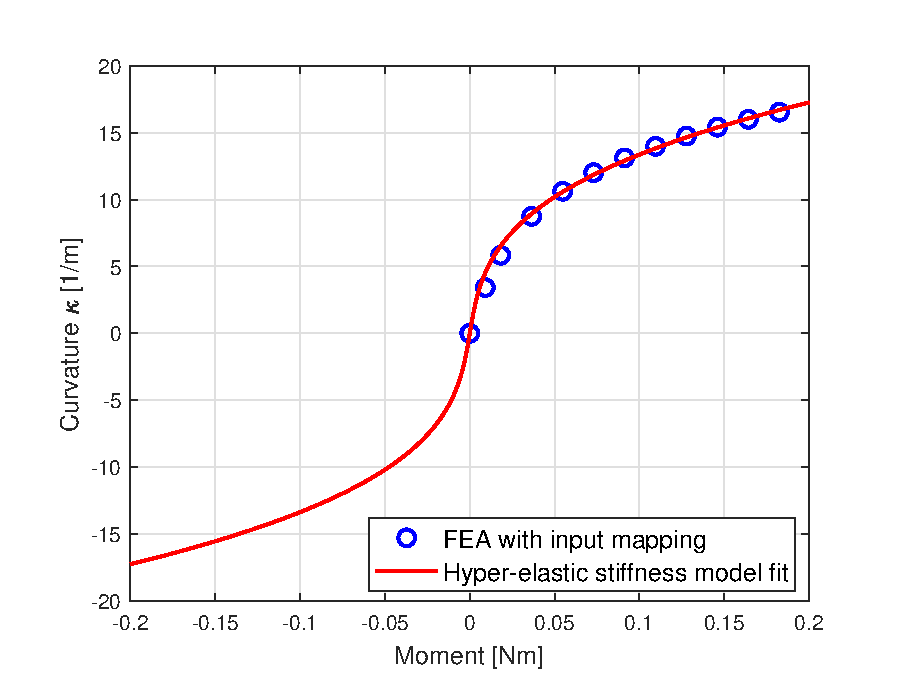
\includegraphics[width=\textwidth]{Figures/Chapter3/mappedmomentvscurvature.eps} 
        \caption{Fitted stiffness model for curvature.}
        \label{fig3:curvsmoment}
    \end{minipage}
\end{figure}


At this point, it should be emphasized that during experimental analysis the soft robot, on which this parameter study is based, was found too porous. This caused excessive air leaks through the walls of the soft robot and therefore was not suitable for further use. Therefore, the methodology of acquiring stiffness data and pressure mapping should be valued instead of the found values. During experimental analysis, a geometric equivalent soft robot is used. However, this robot has thicker walls, reducing its porosity but increasing the stiffness. 




\section{Pump Dynamics}



The pump dynamics have a major contribution to the overall system dynamics. As mentioned, the dynamic model's purpose is to assess and evaluate controller performance. Therefore, it is essential to include the dynamics of the pumps. First, the system's response to a step input is analyzed. This step response contains valuable information regarding the friction of the air pumps. Then, the pressure response is measured for an oscillatory input signal. This data allows us to fit the proposed linear pump model of (\ref{eq2:pumpmodel}).


Previous research conducted on a similar soft robot showed that adding an air vessel between the air pump and soft robot will reduce oscillatory behaviour \cite{proper}. The elastic behaviour of the actuator causes vibrations when the pump injects compressed air into the system. When air is injected into the system, an airwave of higher pressure travels through the soft robot. This causes local pressure variations that are observed by the pressure sensor. This behaviour can be related to the intrinsic characteristics of diaphragm air pumps. Furthermore, the system's volume is not constant. As the soft robot is pressurized, the volume increases, creating a constant interaction between volume and pressure. This interaction is perceived as noise by the pressure sensor. This constant interaction between the elasticity properties of the soft robot and the characteristics of diaphragm pumps can be partly resolved using air tanks. This air tank causes the total control volume to increase, thereby decreasing the relative volume increase caused by inflating the soft robot. Additionally, the local airwaves dissipate faster. The addition of the air vessel, therefore, acts as a low pass filter, reducing high-frequency noise. However, it also reduces the bandwidth as it takes more time to reach the steady-state pressure.

For determining the step response of the system, the pump is connected to an air distribution manifold. To this air distribution manifold, one bellow of the soft robot, the air tank and the pressure sensor are connected. The step response for step inputs between 1 and 9 volt is presented in Figure \ref{fig3:pump_dynamics_adapted}. Although the operating range of the pumps is 12 Volt DC, maximum volt input of 9 volt could be achieved. The system pressure attained for this volt input is theoretically above the pressure sensors limits. Namely, the pressure sensor measures absolute pressures between 0 and 25 PSI, which is equivalent to a maximum of 172 kPa. Depending on weather conditions, the maximum measurable pressure is around 72 kPa, as atmospheric pressure is around 100 kPa. However, experiments have shown that pressures up to 85 kPa can still be measured.  

\begin{figure}[H]
    \centering
    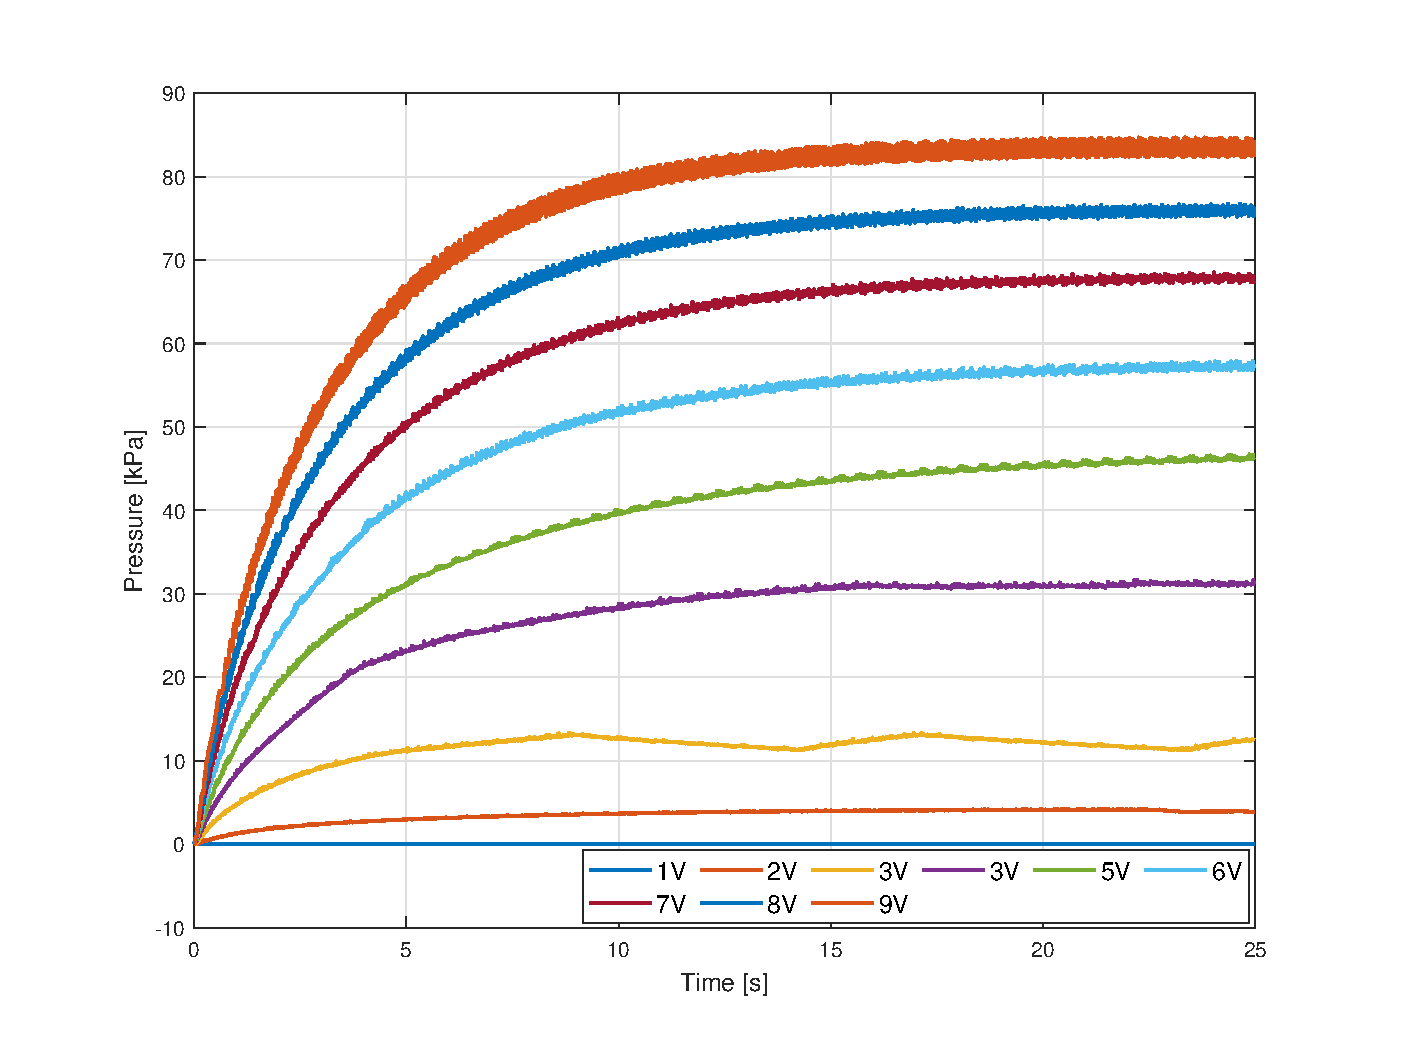
\includegraphics[width = 0.75\textwidth]{Figures/Chapter3/stepnewairtankbellow.eps}
    \caption{Step response for volt step input between 1V and 9V for the system including air vessel and actuator.}
    \label{fig3:pump_dynamics_adapted}
\end{figure}


Multiple observations can be made based on the step response of Figure \ref{fig3:pump_dynamics_adapted}. A first glance reveals first-order system behaviour as pressure increase seems to be proportional to the actual pressure. However, the steady-state pressure is not proportional to the input volt for all inputs. The reason for this behaviour is caused by friction. For 1 and 2 volt input, static friction dominates resulting in almost no pressure change. Between 3 and 4 volts, the transition between dry and kinetic friction is found. Here, the pressure increase is becoming more proportional to the input voltage. From 5 volt onwards the steady-state pressure scales more or less linearly with the input voltage. This coincides with the observation presented in the work of \cite{berkers}, where friction effects were observed below 4.7 volts.

Based on the results of the step response, a time varying input signal can be designed to fit the pump model to. To limit the friction effects a sinusoidal input signal is proposed as,

\begin{equation}
    V(t) =  7 + 2 \sin(2 \pi 0.25t),
    \label{eq3:vinput}
\end{equation}


where the oscillation is around the 7 volt mean, with an amplitude of 2 volt and a frequency of 0.25 Hertz. Using this input signal the dynamic model of (\ref{eq2:pumpmodel}) can be found solving the least square's problem as,

\begin{equation}
   \begin{aligned}
\min_{\lambda_1,\lambda_2} \hspace{5pt}  \Big(\underbar{p}(t) - (-\lambda_1 p(t) +\lambda_2 V(t)\Big)^2   \\ 
\text{s.t.} \hspace{5pt} \lambda_1 > 0 \\
\lambda_2 > 0,
\end{aligned}
\end{equation}

where $\underbar{p}(t)$ is the measured pressure at time instance $t$. Figure \ref{fig3:pumpfit} shows the experimental data and the fitted pump model. The pump parameters found by optimization are $\lambda_1 = 0.2853 [-]$ and $\lambda_2 = 2.6879 \frac{kPa}{V}$. The zoom-in as shown in Figure \ref{fig3:pumpfit} shows a single oscillation. It can be seen that noise amplitude is not constant for an entire oscillation. During pressure increase, the amplitude of the noise is higher, related to the earlier explained phenomena. Since the pump cannot actively deflate, air continuously escapes via the porous walls of the soft robot. During deflation, the input to the air pumps also decreases, thereby reducing noise levels. 
%\newpage

\begin{figure}[H]
    \centering
    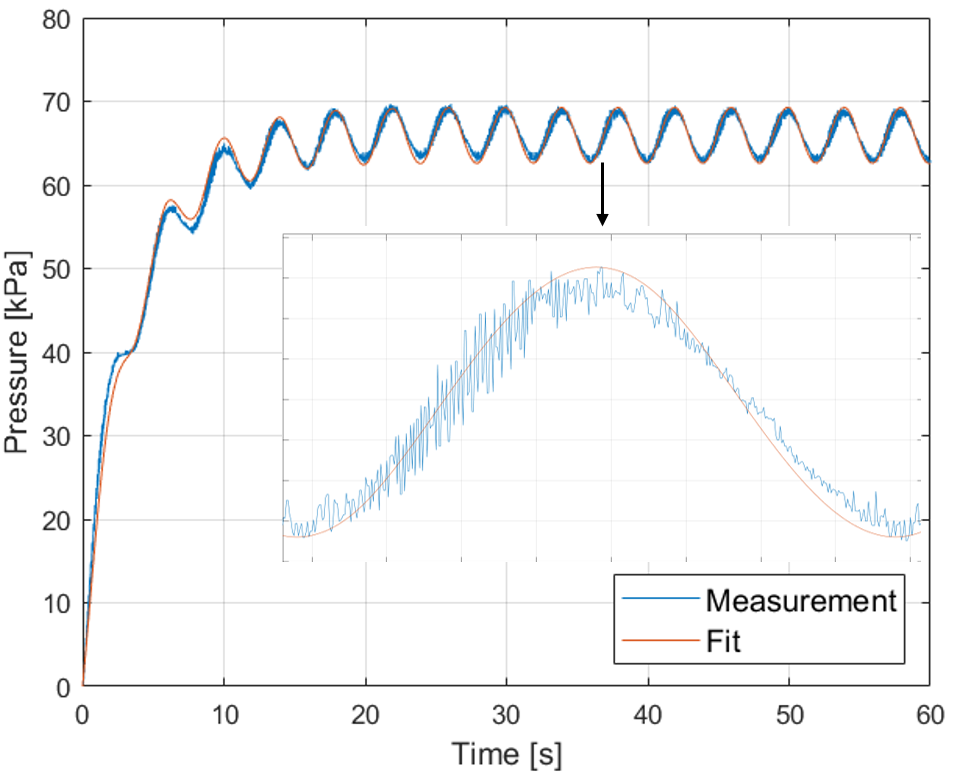
\includegraphics[width = 0.55\textwidth]{Figures/Chapter3/expfitzoom.png}
    \caption{Measured pressure response and pump model fit. Including a zoom-in for one oscillation at 36 seconds.}
    \label{fig3:pumpfit}
\end{figure}


\section*{Summary} 

This chapter comprised a parameter identification on the soft robot's stiffness and pump dynamics. An finite element analysis is conducted to determine the soft robots elongation and rotations for a set of pressures. These pressures are related to force and moment, which allows determining the elongation and rotation stiffness. These stiffnesses are described by a hyper-elastic stiffness model. Furthermore, the pump dynamics are determined. First, a step response is conducted which showed achievable pressures given an input voltage to the air pump. Based on this step response, a sinusoidal input reference signal was designed. The measured pressure response to this input signal allowed determining the pump parameters of the pump model. 

